\section{Detector Packages}
The detector stacks in both spectrometers consist of a lead glass calorimeter,
one or more Cherenkov counters, a hodoscope, and a pair of drift chambers.
Details beyond what are covered here can be found
online~\cite{Standard_Equipment_Manual}.

\subsection{Hodoscopes}

The HMS and SHMS hodoscopes consist of two pairs of X/Y planes
that generate the basic trigger for the DAQ system and provide an initial
estimate of particle velocity based on time of flight (TOF).
Each X (Y) plane consists of some number of horizontally (vertically) oriented
paddles.
All paddles except those in the SHMS S2Y are plastic scintillators.
The HMS paddles are BC-404~\cite{Standard_Equipment_Manual,BC404}.
The SHMS S1X, S1Y, and S2X paddles are RP-408~\cite{SHMS_hodo_plastic,RP408}.
The SHMS S2Y paddles are quartz~\cite{SHMS_hodo_quartz}.
In both spectrometers the first pair of planes, S1X and S1Y, are
about \SI{2.2}{m} upstream from the second pair of planes, S2X and S2Y.
Table~\ref{tab:hodoscope_characteristics} contains a summary of each plane.

\begin{figure}[!h]
    \centering
    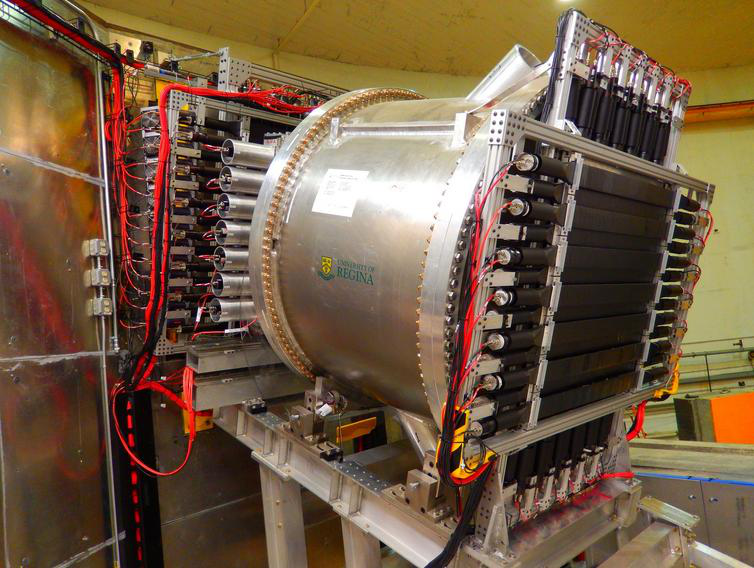
\includegraphics[width=1.0\textwidth]{chap3/shms_hodoscope.png}
    \caption{The two pairs of hodoscope planes that make up the SHMS
             hodoscope are placed on either side of Aerogel and Heavy Gas
             Cherenkov detectors.}
    \label{fig:shms_hodoscope}
\end{figure}

\begin{table}[h]
    \centering
    \caption{Summary of the HMS and SHMS hodoscopes}
    \label{tab:hodoscope_characteristics}
    \resizebox{1.0\textwidth}{!}{
        \begin{tabular}[t]{lcccccccc}
            \hline
            \hline
            Parameter                            & \multicolumn{4}{c}{HMS} & \multicolumn{4}{c}{SHMS} \\
                                                 & S1X & S1Y & S2X & S2Y & S1X & S1Y & S2X & S2Y \\
            \hline

            Width (mm)                           & 8.0 & 8.0 & 8.0 & 8.0 & 8.0 & 8.0 & 10.0 & 5.5 \\
            Thickness (mm)                       & 1.0 & 1.0 & 1.0 & 1.0 & 5.0 & 5.0 & 5.0 & 2.5 \\
            Length (mm)                          & 75.5 & 120.5 & 75.5 & 120.5 & 100.0 & 100.0 & 110.0 & 125 \\
                                                     \\
            z-position (cm)                      & 77.83 & 97.52 & 298.82 & 318.51 & 52.1 & 61.7 & 271.4 & 282.4 \\
            Pitch (cm)                           & 7.5  & 7.5  & 7.5  & 7.5  & 7.5  & 7.5  & 9.5  & 5.0  \\
            $\delta$z from odd numbered          & 2.12 & 2.12 & 2.12 & 2.12 & 2.12 & -2.12 & -2.12 & -5.4 \\
            to even numbered paddles             &   &   &   &   &   &   &   &   \\
                                                     \\
            Paddles per plane                    & 16 & 10 & 16 & 10 & 13 & 13 & 14 & 21 \\
                                                     \\
            Material                             & BC404 & BC404 & BC404 & BC404 & RP408 & RP408 & RP408 & Quartz \\
            \hline
        \end{tabular}
    } % resizebox
\end{table}

Plastic scintillators are solid plastics that contain organic scintillating
compounds: aromatic hydrocarbons containing linked or condensed benzene-ring
structures~\cite{Leo_1994}.
Light produced in plastic scintillators is generated by transitions of free
valence electrons belonging to $\pi$-molecular orbitals.
When a particle passes through the material, it excites electrons to either a
singlet or triplet state, as well as a vibrational mode of the molecule,
as shown in figure~\ref{fig:leo_scintillator_energy_levels}.

\begin{figure}[!h]
    \centering
    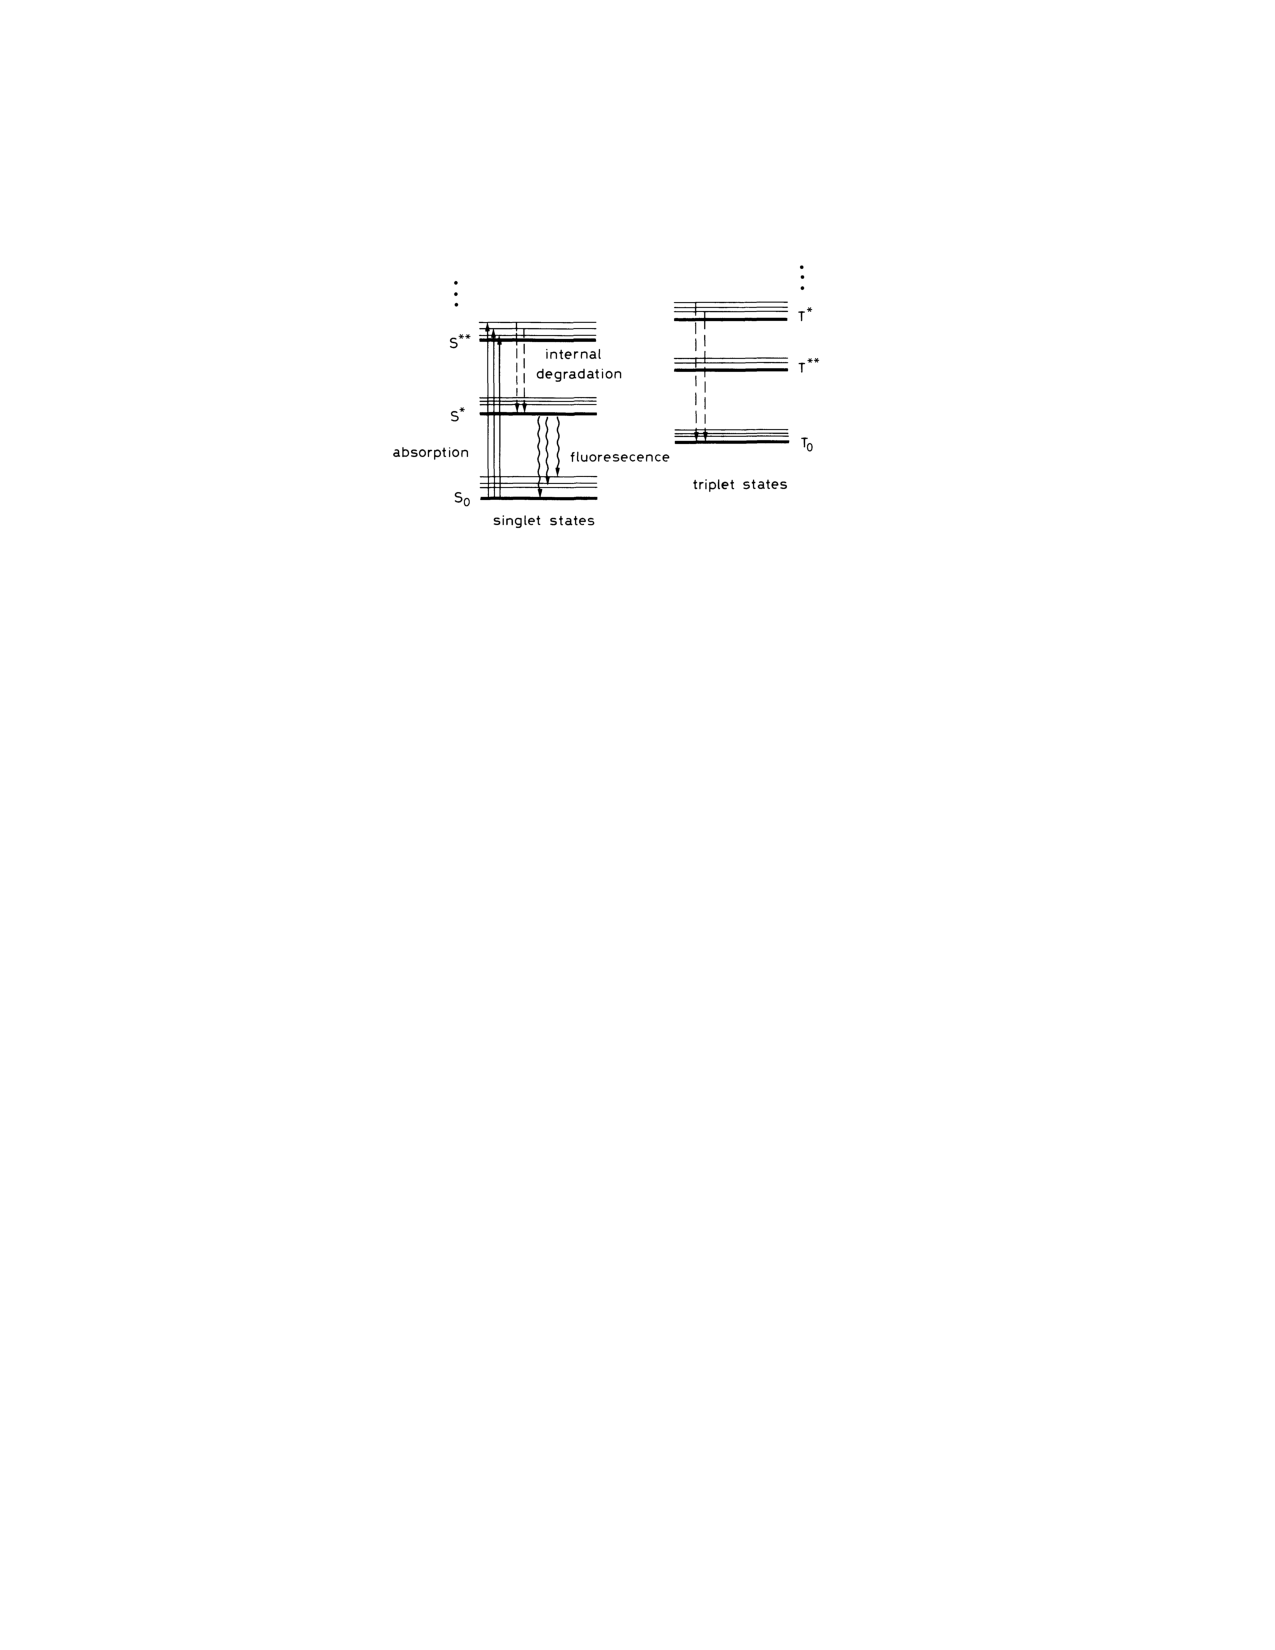
\includegraphics[width=0.6\textwidth]{chap3/leo_scintillator_energy_levels.pdf}
    \caption{A schematic diagram of the energy levels of an organic
             scintillator~\cite{Leo_1994}. Particles passing through the
             material will excite valence electrons to singlet and triplet
             states, decay from which will create visible light.}
    \label{fig:leo_scintillator_energy_levels}
\end{figure}

An electron excited to the $S^{**}$ state will quickly decay to $S^*$ without
radiation, and then radiatively decay to a vibrational state of the ground
state $S_0$ within a few nanoseconds.
The energy of the radiation is less than that required to excite an electron
from $S_0$ to $S^*$, so none of it will be absorbed in the process.
The material is transparent to its own radiation.

The transition from a triplet state is similar.
Decay from $T_0$ to $S_0$ is possible, but suppressed by selection rules.
The decay typically takes place when two $T_0$ molecules interact with each
other, resulting in one in the excited $S^*$ state, one in the ground state,
and heat dissipated in the medium. The excited $S^*$ molecule then rediatively
decays as in the singlet case.

Light produced in the SHMS quartz plane is Cherenkov radiation, which is
discussed further in the subsection on Threshold Chereknov Counters.
% No neutrons produce C rad, so can use S2Y as a veto

Both ends of each HMS paddle are read out by Philips XP2282B PMTs, with
nominal operating voltages of $\sim\SI{1800}{V}$~\cite{HMS_hodoscope_HV}.
Similarly, the ends of each SHMS paddle are read out by a combination of ET
ET9214B, ET ET9814QB, Photonis XP2262B, and Photonis XP2020QB PMTs.
The operating voltages for each SHMS hodoscope PMT are available on the Hall C
Wiki~\cite{SHMS_hodoscope_plastic_HV, SHMS_hodoscope_quartz_HV}.

The signals from each PMT are fed into a passive splitter, yielding two signals
with amplitudes 1/3 and 2/3 of the original.
The smaller signal is sent to a flash Analog-to-Digital Converter (fADC).
The larger is sent to a discriminator as part the core of the trigger system,
which will be discussed in the next section.

\subsection{Drift Chambers}
\label{subsection:drift_chambers}
Both spectrometers have a pair of drift chambers~\cite{SHMS_drift_chambers}
that provide precise tracking information.
Combined with knowledge of the spectrometers' optics, this tracking information
is used to calculate particle momenta, angles, and positions at the interaction
point in the target.

\begin{figure}[!h]
    \centering
    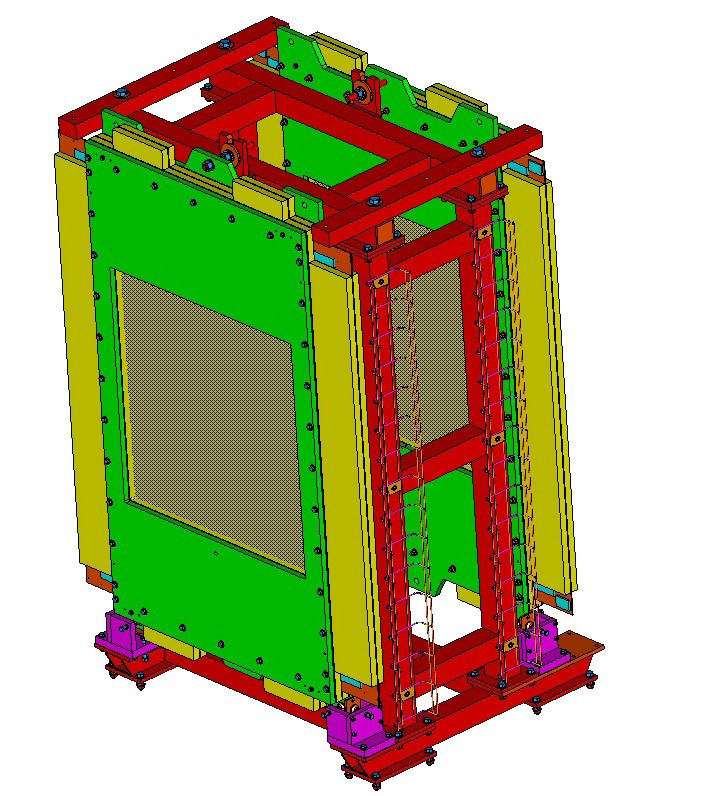
\includegraphics[width=0.6\textwidth]{chap3/shms_dc.png}
    \caption{A rendering  of the SHMS drift chambers mounted in the detector
             hut frame.}
    \label{fig:shms_dc}
\end{figure}

The drift chamber packages consist of a pair of identical chambers, each of
consists of six wire planes.
Each chamber has an active area of 80x80\si{\cm\squared} to match the size of
the SHMS's acceptance and focal plane.
Copper-coated mylar cathode planes are placed between each wire plane, before
the first plane, and after the last plane.
Each wire plane consists of a set of alternating \SI{20}{\micro\meter} gold
tungsten sense (anode) wires and \SI{80}{\micro\meter} field wires, separated
by \SI{500}{\micro\meter}.
To reduce cost, only two wire orientations were manufactured: an X plane with
horizontally oriented wires and a U plane with wires oriented 60$^{\circ}$ from
the X wires, both of which are shown in figure~\ref{fig:dc_planes}.
In the SHMS, the U planes have 109 sense wires per plane and the X planes have
79.
In the HMS, the U planes have 96 sense wires per plane and the X planes have
102.

\begin{figure}[h]
    \centering
    \begin{subfigure}[b]{0.4\textwidth}
        \centering
        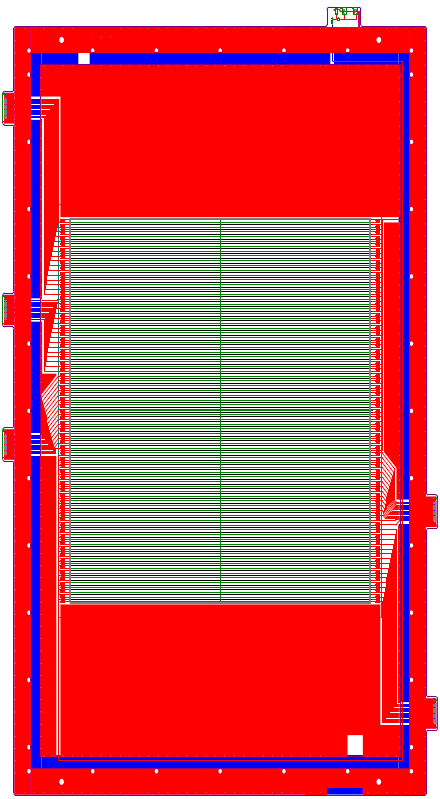
\includegraphics[width=\textwidth]{chap3/shms_dc_x_plane.png}
        \caption{X plane}
        \label{fig:dc_x_plane}
    \end{subfigure}
    \hfill
    \begin{subfigure}[b]{0.4\textwidth}
        \centering
        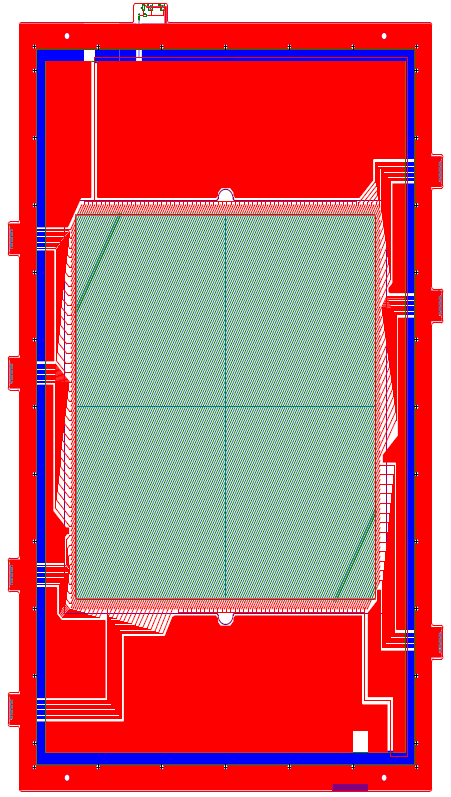
\includegraphics[width=\textwidth]{chap3/shms_dc_u_plane.png}
        \caption{U plane}
        \label{fig:dc_u_plane}
    \end{subfigure}
    \caption{The drift chambers consist of 6 wire planes with different
             orientations, each of which are generated by rotating the two
             X and U planes.}
    \label{fig:dc_planes}
\end{figure}

X' and U' planes, with identical wire orientations offset by
\SI{500}{\micro\meter} from the unprimed planes, can be generated by rotating
an X or U plane 180$^\circ$ such that the top becomes the bottom.
V and V' planes, with wires oriented -60$^\circ$ from the X wires, can be
generated by rotating the U and U' planes 180$^\circ$ around a vertical axis
running through the center of the plane.
The offset between the primed and unprimed planes allows us to resolve the
left-right ambiguity of each hit\footnote{For a hit on an isolated drift
chamber wire, it is impossible to know whether the ionized electrons came from
the right or the left of the wire. This will be discussed further in the
chapter on data analysis.}

\begin{figure}[!h]
    \centering
    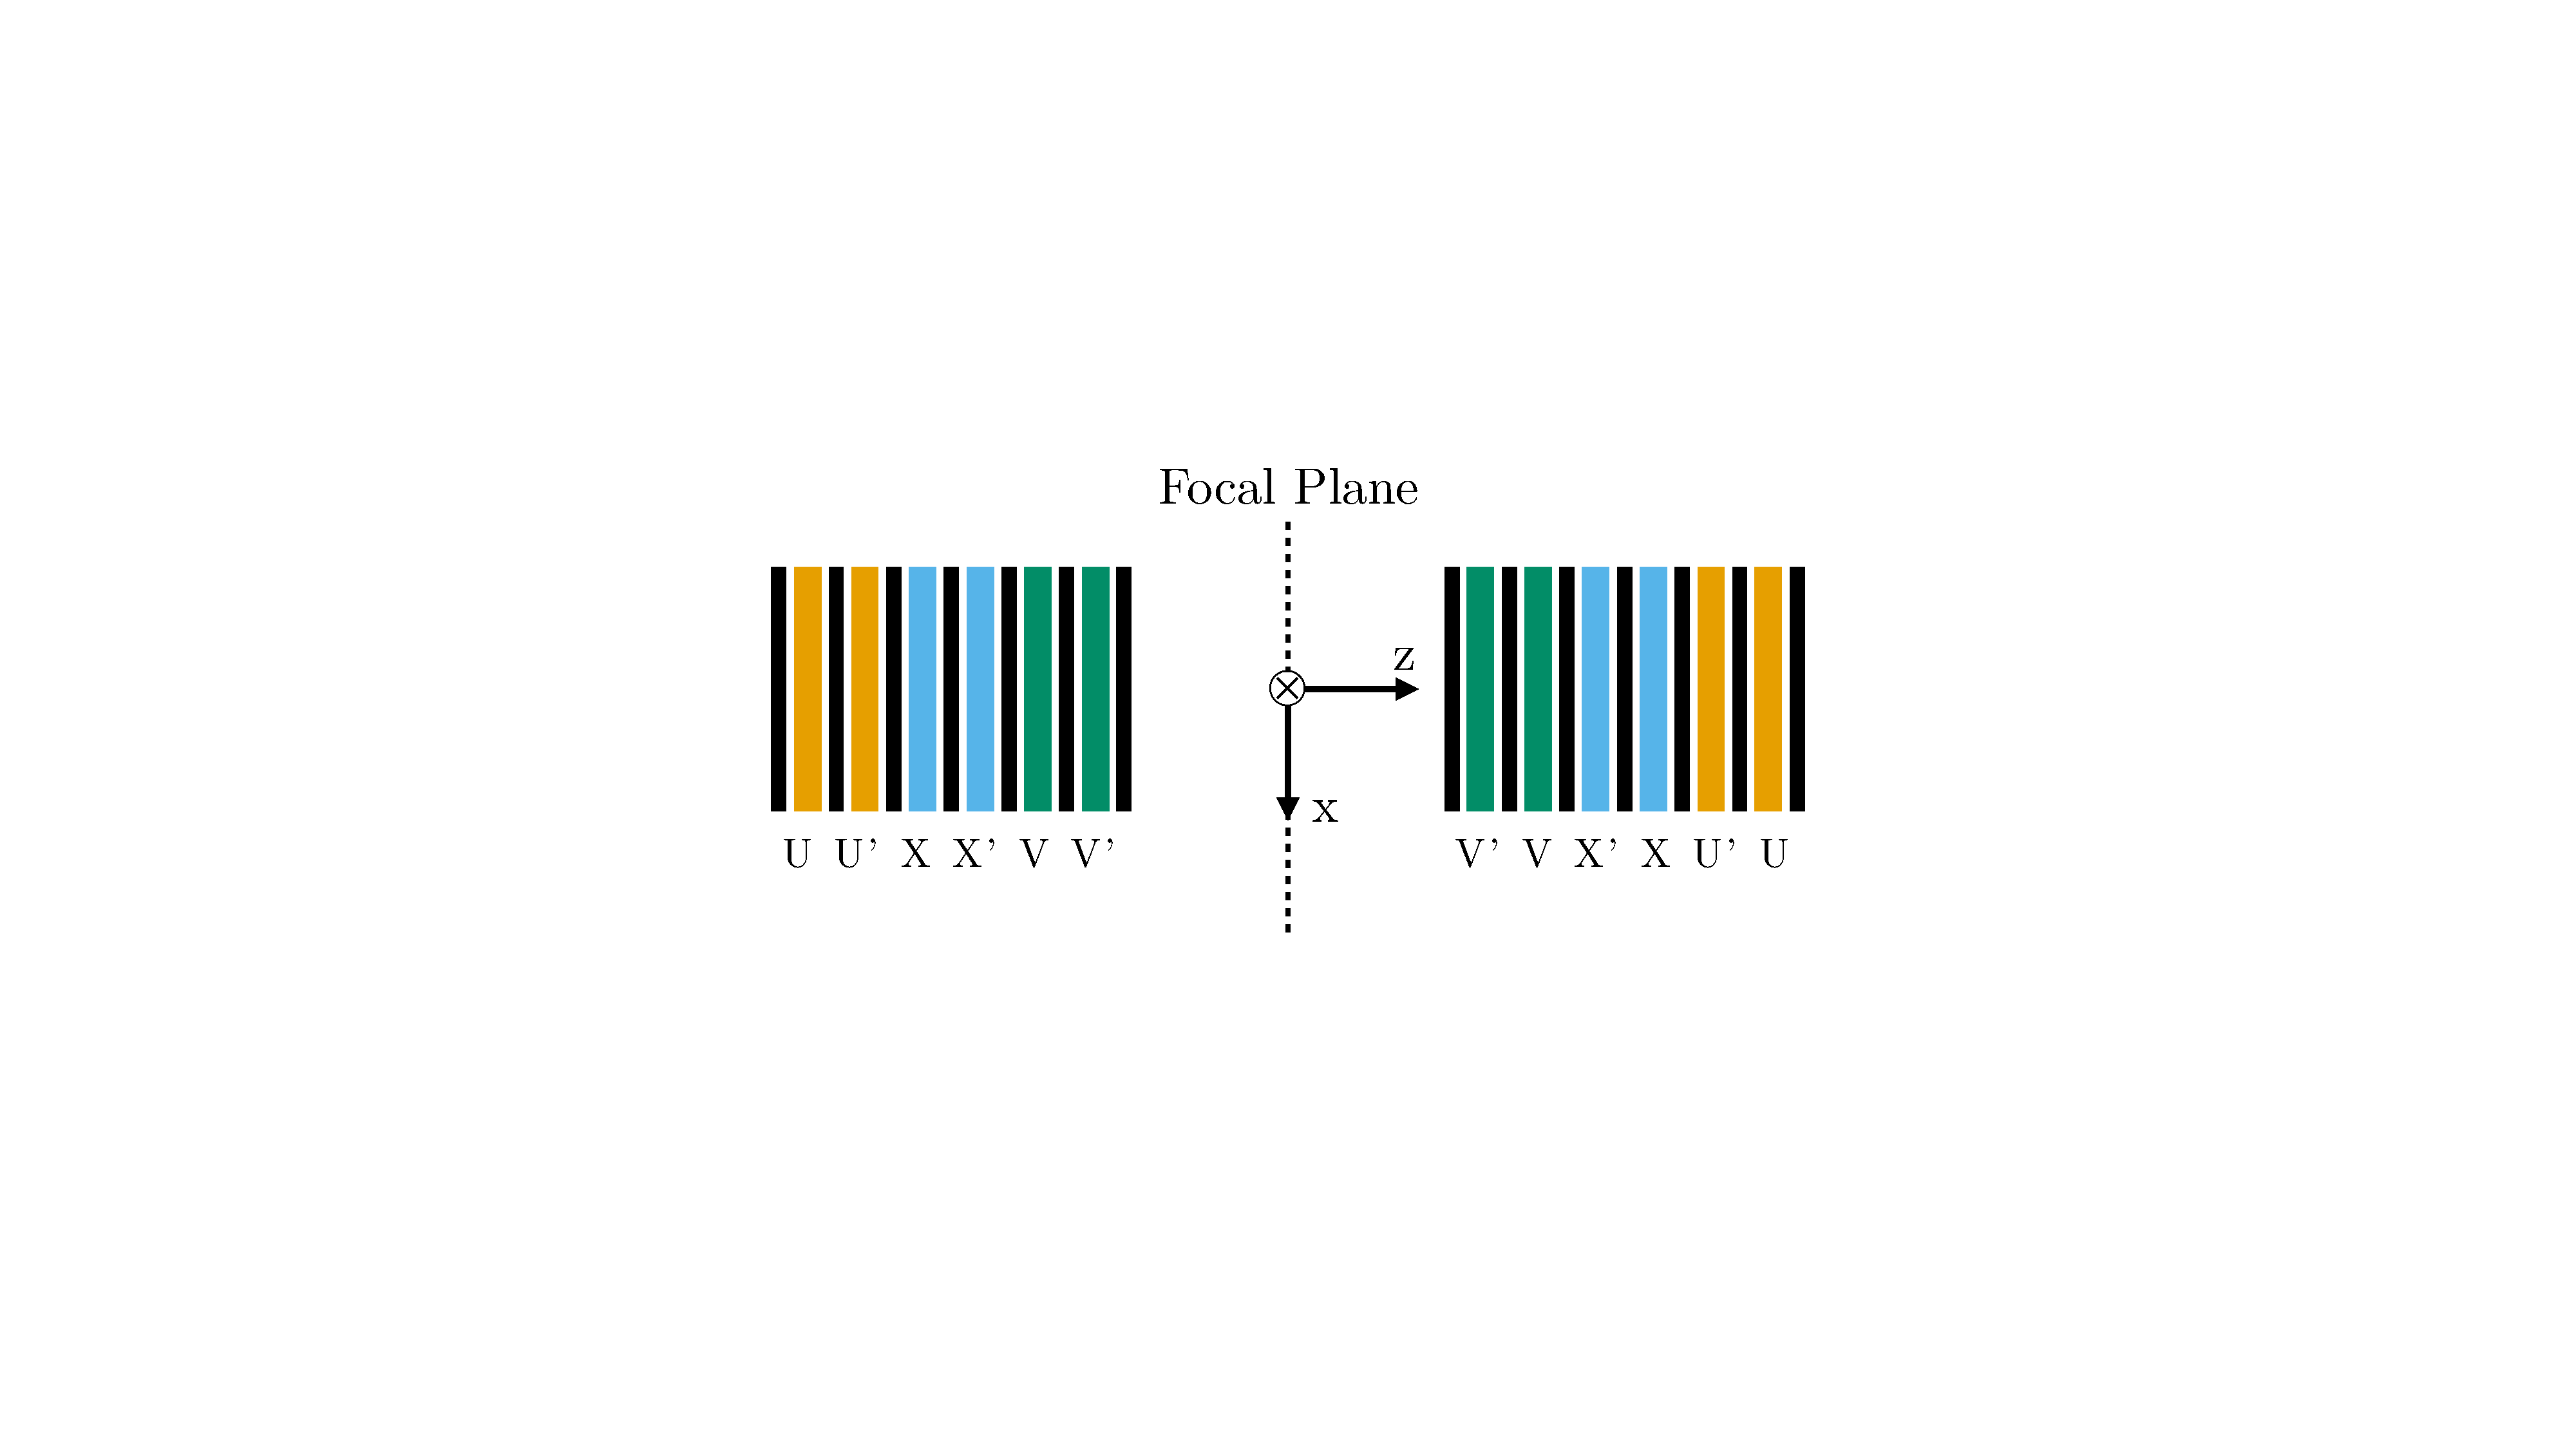
\includegraphics[width=0.6\textwidth]{chap3/dc_plane_order.pdf}
    \caption{Side view of the order of planes encountered by a particle
             traveling through the SHMS. The focal plane of the spectrometer
             is roughly halfway between the two drift chambers.}
    \label{fig:shms_plane_order}
\end{figure}

As shown in figure~\ref{fig:shms_plane_order}, the order of the planes in the
first chamber encountered by a particle traveling through the SHMS is
(U,U',X,X',V,V').
The order in the second chamber is reversed.
In the HMS, the V and V' planes in each chamber are swapped.

During operation, each chamber is filled with a 50/50 mix of argon and ethane.
When a charged particle passes through the chamber, it will ionize some of
the gas.
The cathode planes and field wires are kept at $\sim-\SI{1900}{V}$ with respect
to the sense wires kept at ground, creating an electric field pointing from
sense wires toward field wires and cathode planes.
The field accelerates these primary ionized electrons toward the sense wires,
ionizing more electrons along the way.
The resulting cloud of electrons drifts toward sense wires at a
constant ``drift velocity.''

The electrons are collected by sense wires which are read out by
16-channel discriminators attached to the chamber supports.
The discriminators are fed, via 16-channel ribbon cables, to CAEN 1190
TDCs~\cite{CAEN_1190_manual} in a VXS crate in the detector huts.
When the 1190s receive a pre-trigger, they record the time of the last several
hits\footnote{The trigger and readout electronics will be discussed in more
detail in the next section.}.
The time between the pre-trigger and the time at which the electron cloud hits
a wire can be used to determine the distance at which the initial ionization
occurred.
Using this information from every wire plane in both chambers allows
precise track reconstruction with residuals of \SI{250}{\micro\meter} in the
SHMS and (\SI{350}{\micro\meter} in the HMS.
The complete process of converting raw signals from each wire to full tracking
information will be discussed in section~\ref{section:daq}.

\subsection{Threshold Cherenkov Counters}
Threshold Cherenkov counters make use of a particle-dependent Cherenkov
radiation threshold to discriminate between types of particles.
A charged particle with mass $m$, velocity $\beta$, and 3-momentum $p$ passing
through a medium with index of refraction $n$ will emit Cherenkov radiation if
\begin{equation}
    \frac{c}{n} < \beta = \frac{p}{\sqrt{p^2+m^2}}
\end{equation}
or equivalently, as illustrated in figure~\ref{fig:hms_cer_threshold},
\begin{equation}
    1-\frac{c}{data,dtwsjkjkn} > 1-\beta = 1-\frac{p}{\sqrt{p^2+m^2}}
\end{equation}

% HMS has C4F8O at 0.45 atm.  % n=1.00137 @ 1 atm per https://userweb.jlab.org/~hcf/shmsnim/shmsNIM.pdf
\begin{figure}[!h]
    \centering
    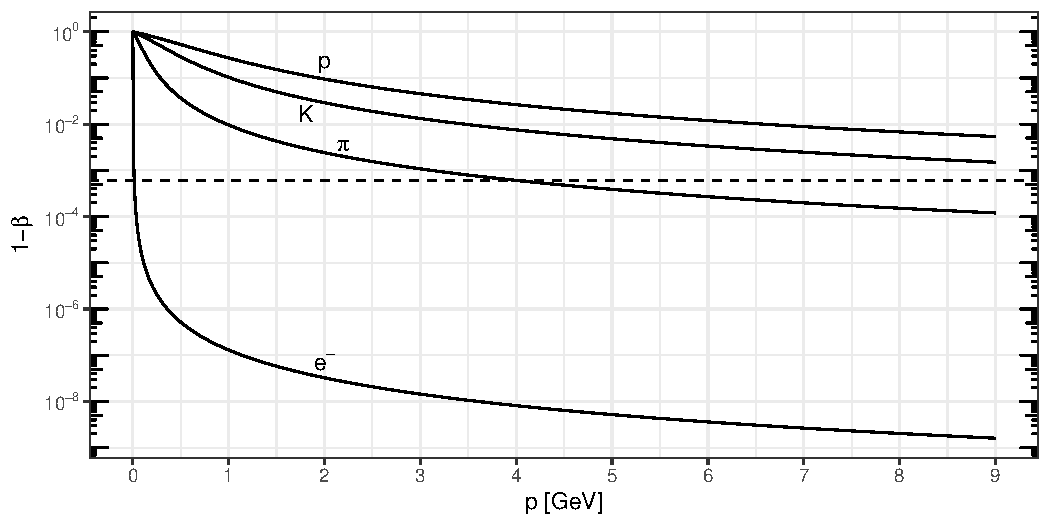
\includegraphics[width=1.0\textwidth]{chap3/hms_cer_threshold.pdf}
    \caption{Value of $1-\beta$ for various particles as a function of
            momentum. The horizontal line represents the Cherenkov threshold
            for \ch{C4F8O} at a pressure of 0.45 atm, below which a particle
            will produce Cherenkov radiation. TODO: add labels to gases.
            }
    \label{fig:hms_cer_threshold}
\end{figure}

Over a sufficiently narrow range of momenta, only some types of particles will
emit Cherenkov radiation.
For example, for a threshold Chereknov counter filled with \ch{C4F8O} at
0.45 atm, the presence or absence of Cherenkov radiation can be used to
determine if the particle that generated a trigger is an electron or a hadron,
provided the momentum range in question is below $\sim$4 \si{\giga\eV}.
Given knowledge of the expected range of momenta an experiment requires and
what types of backgrounds will need to be removed, one can pick an appropriate
Cherenkov medium based on its index of refraction. Further tuning of the
threshold can be done by adjusting the pressure of the gas, making use of
the fact that pressure is proportional to $n-1$.

% TODO: make ggplot label gases' thresholds
\begin{figure}[!h]
    \centering
    \includegraphics[width=1.0\textwidth]{chap3/cer_gas_thresholds.pdf}
    \caption{Value of $1-\beta$ for various particles as a function of
            momentum. The horizontal lines represent the Cherenkov threshold
            for various gases at 1 atm, below which a particle
            will produce Cherenkov radiation.
            }
    \label{fig:cer_gas_threshold}
\end{figure}

Suppose a threshold Cherenkov detector has
light-gathering efficiency $\epsilon_c(\lambda)$,
a PMT with quantum efficiency $QE(\lambda)$,
and is filled with a gas with transparency $G(\lambda)$
and index of refraction $n$.
It can be shown~\cite{NGC_Design_Report} that by a particle of charge $e$ passing through the detector
with velocity $\beta$ and path length $L$ will generate
$N_e =AL\left(1-\frac{1}{\beta^2n^2}\right)$ photoelectrons, where
\begin{equation}
A = 2 \pi \alpha \int_{\lambda_1}^{\lambda_2} \epsilon_c(\lambda)QE(\lambda)G(\lambda)\frac{d\lambda}{\lambda^2}.
\end{equation}

The gas Cherenkov detectors in the HMS and SHMS use spherical mirrors to focus
Cherenkov radiation onto PMTs mounted on the back of the detector. The SHMS
aerogel Cherenkov consists of an aeorogel tray, covered in either GORE or
Millipore diffusion materials~\cite{Horn_2017}, mounted between two columns
of PMTs.

\subsubsection{HMS Cherenkov}
% Some leads for hunting down the original article. Could just ask Donal
% https://www.osti.gov/biblio/374934
% http://flux.aps.org/meetings/YR9596/BAPSAPR95/abs/SJ0805.html
% https://uva.worldcat.org/title/a-threshold-gas-cerenkov-detector-for-cebafs-hall-c-high-momentum-spectrometer/oclc/4436255400?referer=brief_results

\begin{figure}[ht]
    \centering
    \begin{subfigure}[b]{0.4\textwidth}
        \centering
        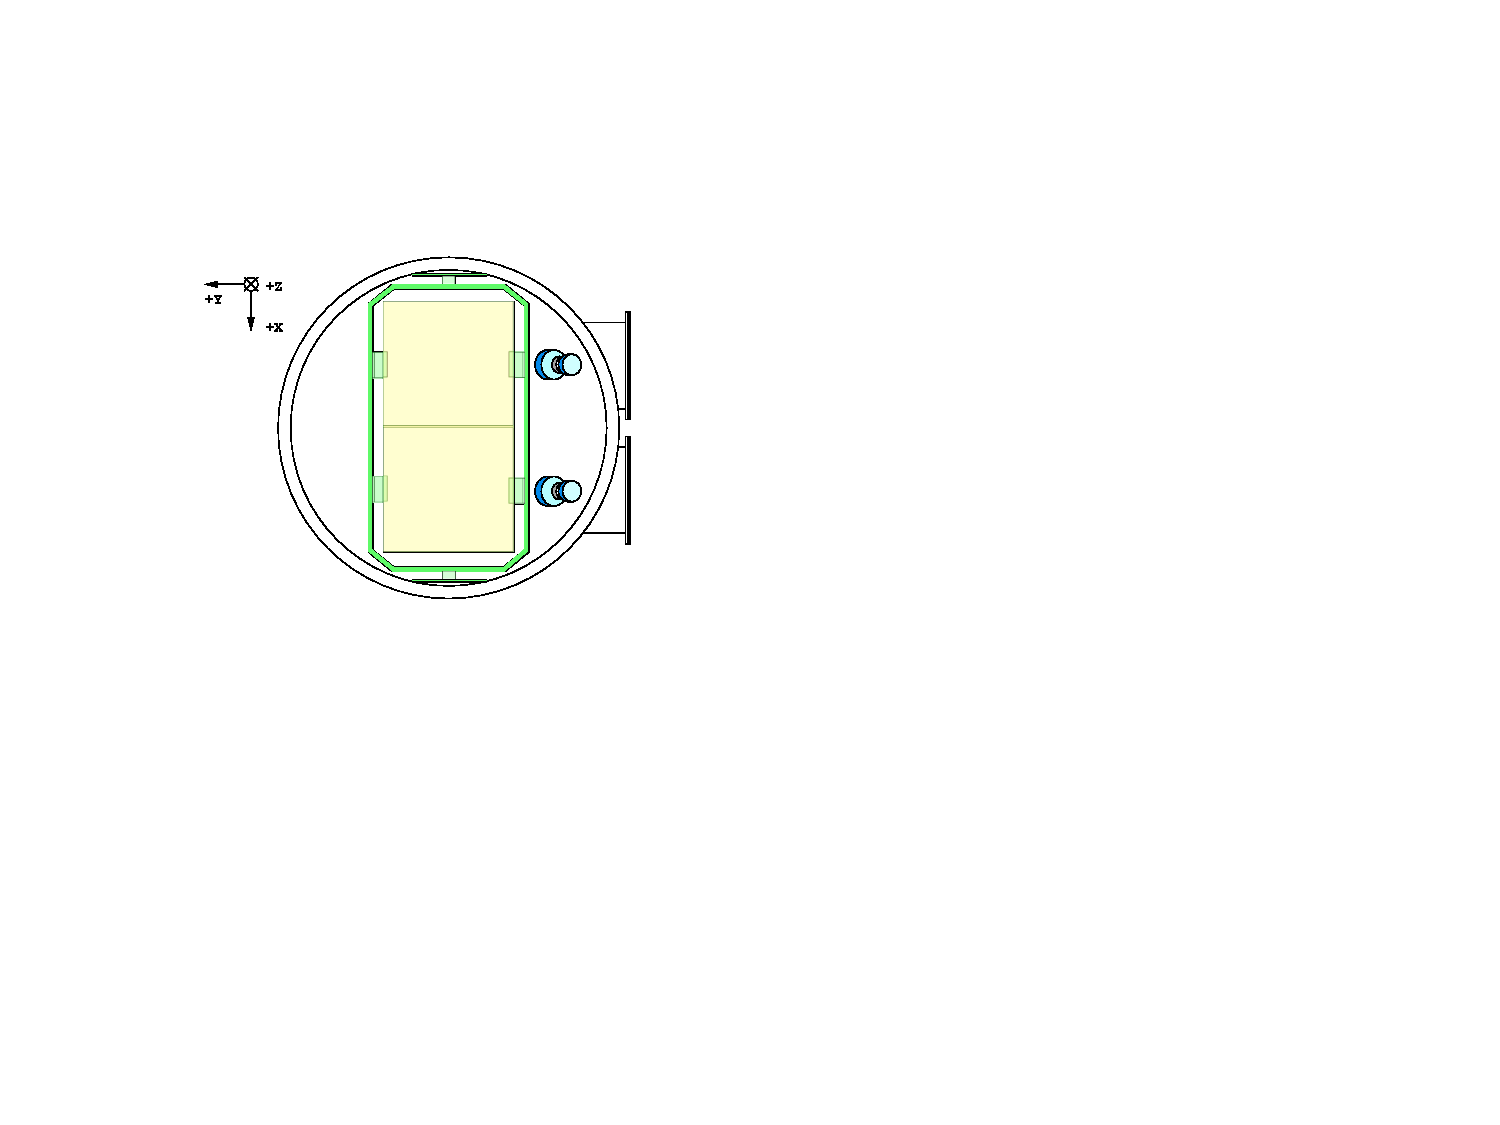
\includegraphics[width=\textwidth]{chap3/hms_cer_front.pdf}
        \caption{Front view}
        \label{fig:hms_cer_front}
    \end{subfigure}
    \hfill
    \begin{subfigure}[b]{0.4\textwidth}
        \centering
        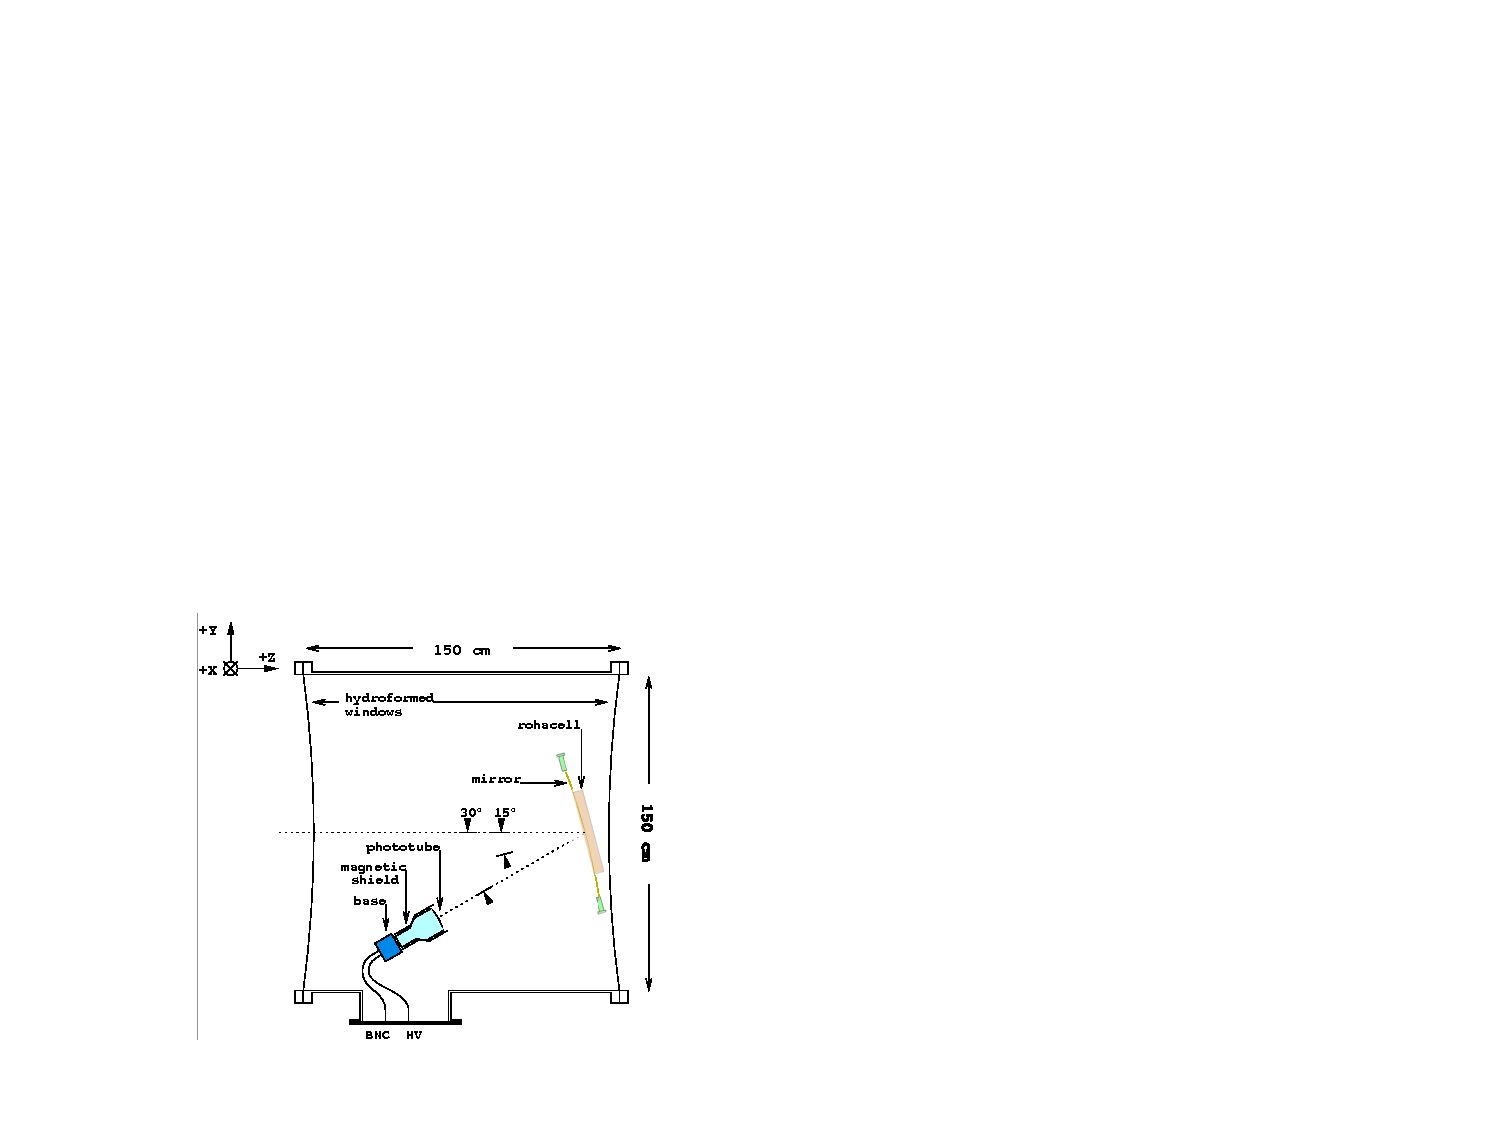
\includegraphics[width=\textwidth]{chap3/hms_cer_top.pdf}
        \caption{Top view}
        \label{fig:hms_cer_top}
    \end{subfigure}
    \caption{The HMS Cherenkov}
    \label{fig:hms_cherenkov}
\end{figure}

The HMS Cherenkov~\cite{Cothran_1995} is designed for electron-pion separation.

During our runs, it was filled with \ch{Ci4F80} at 0.45 atm.

Broken mirror during our runs. Will discuss diagnosis in later section.

\subsubsection{SHMS Noble Gas Cherenkov}
\begin{figure}[ht]
    \centering
    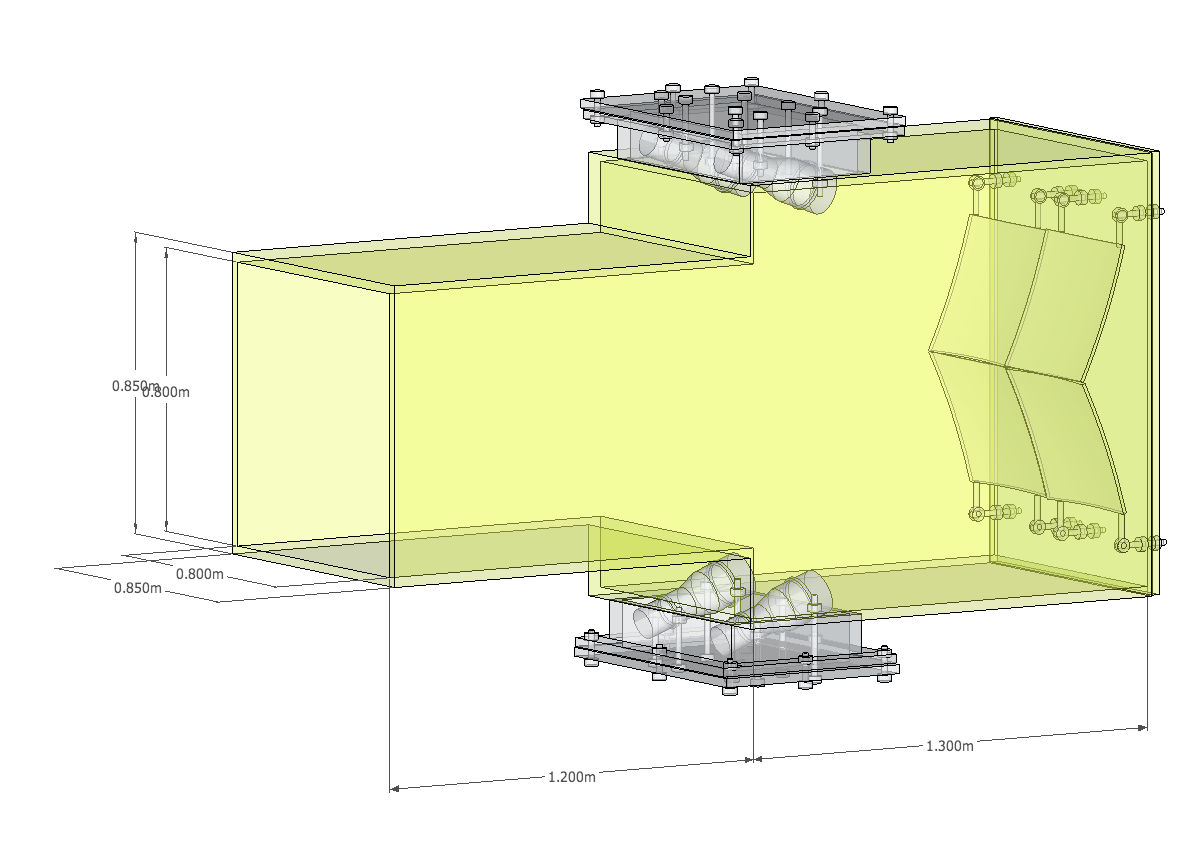
\includegraphics[width=1.0\textwidth]{chap3/shms_ngc_render.png}
    \caption{The SHMS Noble Gas Chereknov }
    \label{fig:shms_ngcer}
\end{figure}

% CO2 at 1 atm.
The SHMS Noble Gas Cherenkov~\cite{NGC_Design_Report} is designed for e/pi
separation.

During our runs, it was filled with \ch{CO2} at 1 atm.

\subsubsection{SHMS Heavy Gas Cherenkov}
\begin{figure}[ht]
    \centering
    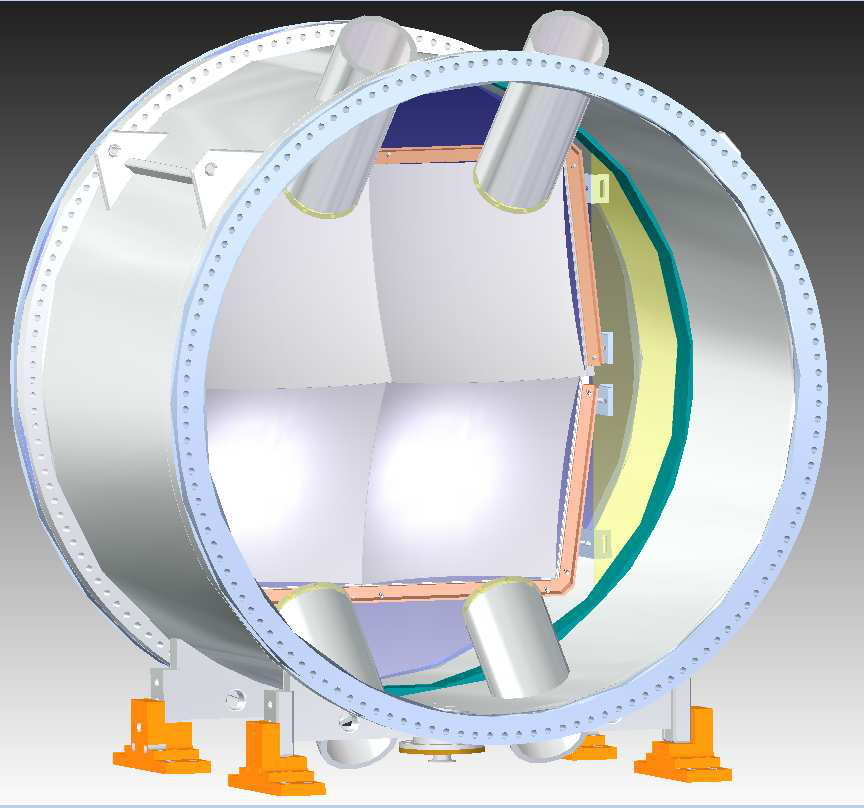
\includegraphics[width=0.5\textwidth]{chap3/shms_hgc_render.png}
    \caption{The SHMS Heavy Gas Chereknov }
    \label{fig:shms_hgcer}
\end{figure}

% CO2 at 1 atm.
Designed for pi/K separation.

During our runs, it was filled with \ch{CO2} at 1 atm.

\subsubsection{SHMS Aerogel Cherenkov}
\begin{figure}[ht]
    \centering
    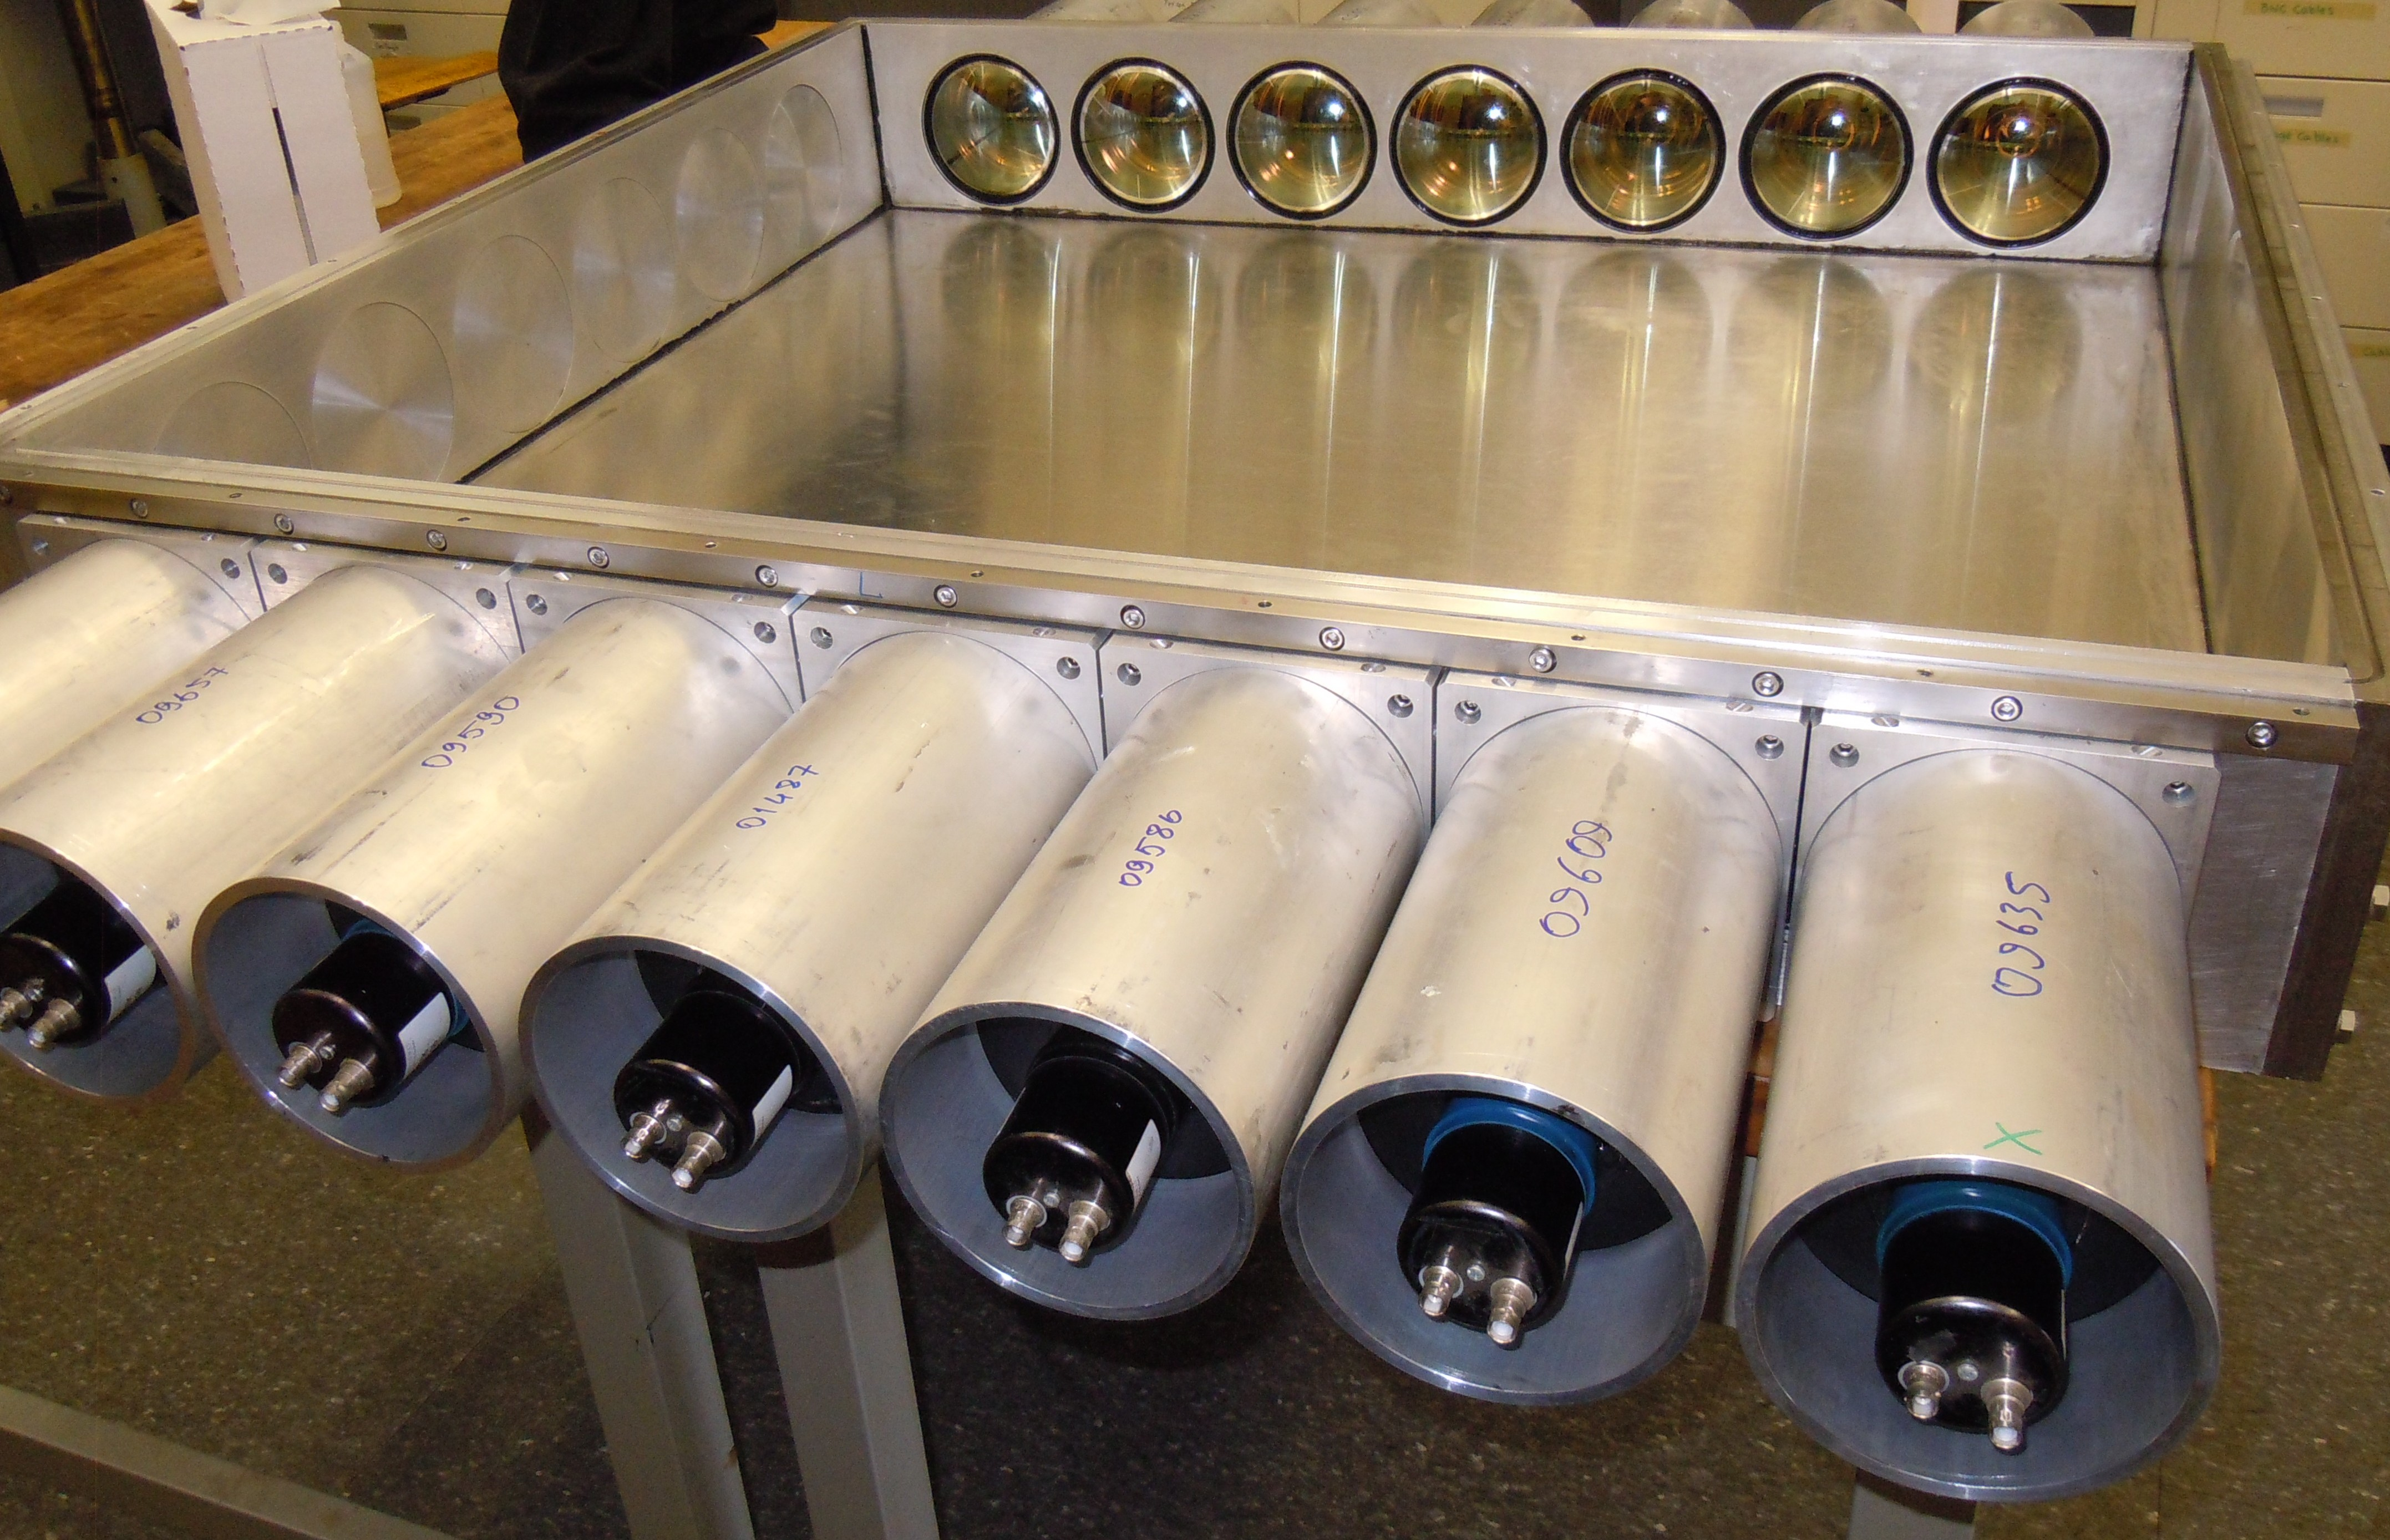
\includegraphics[width=0.5\textwidth]{chap3/shms_aerogel_open.jpg}
    \caption{The SHMS Aerogel Chereknov }
    \label{fig:shms_aerogel}
\end{figure}

The SHMS Aerogel Cherenkov~\cite{Horn_2017} was designed for K/p separation.

\subsection{Calorimeters}
A lead glass calorimeter provides another means for discriminating between
electrons and hadrons.
The calorimeters in both spectrometers consist of lead blocks with
PMTs attached that collect light generated by electromagnetic showers.
The electric field of the nuclei in the block will slow down a high energy
electron passing through the block.
The electron will radiate Bremsstrahlung photons, which will in turn generate
positron-electron pairs that will also radiate photons, and so on.
The resulting electromagnetic shower of photons, electrons, and positrons
generates Cherenkov radiation that is collected by PMTs mounted on the ends
of the lead glass blocks.
The amount of light collected is proportional to the deposited energy.
Electrons, positrons, and photons will deposit all of their energy.
For the kinematics of E12-06-102, this is between 2 and 6 GeV.
These particles will produce a peak centered around 1 in the distribution of
the track-normalized energy deposition, $E/p$.
A pion, whose mass is much greater than an electron's, will typically deposit
about 300 MeV.
A negative pion undergoing a charge-exchange reaction in the bulk of the
calorimeter can produce a neutral pion which will decay into two photons,
resulting in a significant fraction of energy being deposited.
As a result, there is a large pion tail in the $E/p$ distribution that extends
up to 1.
Heavier hadrons typically deposit no energy.

\begin{figure}[ht]
    \centering
    \begin{subfigure}[b]{0.35\textwidth}
        \centering
        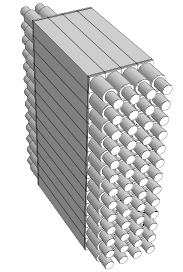
\includegraphics[width=\textwidth]{chap3/hms_calorimeter_drawing_lores.png}
        \caption{HMS calorimeter}
        \label{fig:hms_calorimeter}
    \end{subfigure}
    \hfill
    \begin{subfigure}[b]{0.35\textwidth}
        \centering
        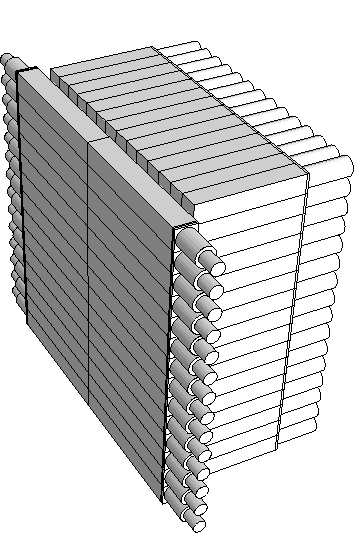
\includegraphics[width=\textwidth]{chap3/shms_calorimeter_drawing.png}
        \caption{SHMS calorimeter}
        \label{fig:shms_calorimeter}
    \end{subfigure}
    \caption{The HMS and SHMS calorimeters}
    \label{fig:calorimeters}
\end{figure}

\subsubsection{HMS Calorimeter}
The HMS calorimeter~\cite{Mkrtchyan_2012} consists of four rows of thirteen
10x10x70 \si{\cm\cubed} lead glass blocks.
The total thickness is $\sim$14.6 radiation lengths.
The blocks are made of TF-1 type lead glass with an index of refraction of
1.65, radiation length 2.74 \si{cm}, and density 3.86 \si{\gram\per\cm\cubed}..
Each block is wrapped in 25 \si{\um} thick aluminized Mylar and 40
\si{\um} thick Tedlar type film to block external light.
The light generated in each block is collected by two Phillips XP3462B PMTs,
one on each end.

\subsubsection{SHMS Calorimeter}
The SHMS calorimeter consists of a preshower and shower section.
The preshower radiator consists of one layer of 28 TF-1 type lead glass blocks,
identical to the HMS blocks, stacked in two columns of 14 blocks.
The ``fly eye'' shower array consists of 224 modules from the decommissioned
HERMES detector~\cite{Avakian_1998} stacked in 14 columns and 16 rows.
The HERMES blocks are 8.9x8.9x50 \si{\cm\cubed} blocks of F-101 type lead glass with
an index of refraction of 1.65, radiation length 2.78 \si{\cm}, and density
3.86 \si{\gram\per\cm\cubed}.
Each preshower block is read out by one Phillips XP3462B PMT, and each shower
block by one Photonis XP3461 PMT.
